\documentclass[11pt,oneside]{article}
\usepackage[T1]{fontenc}
\usepackage[utf8]{inputenc}
%\DeclareUnicodeCharacter{00A0}{ }
\usepackage[adobe-utopia]{mathdesign}

\usepackage{amsmath}
\usepackage[francais]{babel}
\usepackage[dvips]{graphicx}
%\usepackage{here}
\usepackage{framed}
\usepackage[normalem]{ulem}
\usepackage{fancyhdr}
\usepackage{titlesec}
\usepackage{vmargin}

\usepackage{amsmath}
\usepackage{ifthen}
\usepackage{multirow}
\usepackage{multicol} % Portions de texte en colonnes

%\usepackage{xltxtra} % Logo XeLaTeX
%\usepackage{pst-solides3d}
\usepackage{color}
%\usepackage{colortbl}
\usepackage{titletoc} % Pour la mise en forme de la table des matières

%\usepackage[crop=off]{auto-pst-pdf}
%\usepackage{bclogo}


%\usepackage{longtable}
%\usepackage{flafter}%floatants après la référence
%\usepackage{pst-solides3d}
%\usepackage{pstricks}
%\usepackage{minitoc}
%\setcounter{minitocdepth}{4}
%\usepackage{draftcopy}% "Brouillon"
%\usepackage{floatflt}
%\usepackage{psfrag}
%\usepackage{listings} % Permet d'insérer du code de programmation
%\usepackage{lmodern}
%\usepackage[adobe-utopia,uppercase=upright,greeklowercase=upright]{mathdesign}
%\usepackage{minionpro}
%\usepackage{pifont}
%\usepackage{amssymb}
%\usepackage[francais]{varioref}

\setmarginsrb{1.5cm}{1cm}{1cm}{1.5cm}{1cm}{1cm}{1cm}{1cm}

\definecolor{gris25}{gray}{0.75}
\definecolor{bleu}{RGB}{18,33,98}
\definecolor{bleuf}{RGB}{42,94,171}
\definecolor{bleuc}{RGB}{231,239,247}
\definecolor{rougef}{RGB}{185,18,27}
\definecolor{rougec}{RGB}{255,230,231}
\definecolor{vertf}{RGB}{103,126,82}
\definecolor{vertc}{RGB}{220,255,191}
\definecolor{violetf}{RGB}{112,48,160}
\definecolor{violetc}{RGB}{230,224,236}
\definecolor{jaunec}{RGB}{220,255,191}

\usepackage[%
    pdftitle={SLCI -- Modélisation par schémas blocs -- TD},
    pdfauthor={Xavier Pessoles},
    colorlinks=true,
    linkcolor=blue,
    citecolor=magenta]{hyperref}



% \makeatletter \let\ps@plain\ps@empty \makeatother
%% DEBUT DU DOCUMENT
%% =================
\sloppy
\hyphenpenalty 10000

\newcommand{\Pointilles}[1][3]{%
\multido{}{#1}{\makebox[\linewidth]{\dotfill}\\[\parskip]
}}


\begin{document}


\newboolean{prof}
\setboolean{prof}{false}
%------------- En tetes et Pieds de Pages ------------
\pagestyle{fancy}
\renewcommand{\headrulewidth}{0pt}

\fancyhead{}
\fancyhead[L]{%
\noindent\noindent\begin{minipage}[c]{2.6cm}
%Lycée Rouvière PTSI

\includegraphics[width=2cm]{png/logo_ptsi.png}%
\end{minipage}
}

\fancyhead[C]{\rule{12cm}{.5pt}}

\fancyhead[R]{%
\begin{minipage}[c]{3cm}
\begin{flushright}
\footnotesize{\textit{\textsf{Sciences Industrielles\\ de l'Ingénieur}}}%
\end{flushright}
\end{minipage}
}

\renewcommand{\footrulewidth}{0.2pt}

\fancyfoot[C]{\footnotesize{\bfseries \thepage}}
\fancyfoot[L]{\footnotesize{2013 -- 2014} \\ X. \textsc{Pessoles}}
\ifthenelse{\boolean{prof}}{%
\fancyfoot[R]{\footnotesize{CI 2 : SLCI -- Travail Dirigé} \\ \footnotesize{Ch. 3 : Modélisation -- P}}
}{%
\fancyfoot[R]{\footnotesize{CI 2 : SLCI -- Travail Dirigé} \\ \footnotesize{Ch. 3 : Modélisation -- E}}
}


%\begin{center}
%\textit{Centre d'intérêt}
%\end{center}



\begin{center}
 \Large\textsc{CI 2 -- SLCI : Étude du comportement des Systèmes Linéaires Continus Invariants}
\end{center}

\begin{center}
 \large\textsc{Chapitre 3 -- Modélisation des Systèmes Linéaires Continus Invariants}

 \large\textsc{Modélisation par schémas blocs} 
\end{center}

\begin{center}
\textsc{Travail Dirigé} 

\end{center}

\begin{flushright}
\textit{D'après ressources de Florestan Mathurin} 
\end{flushright}
\vspace{.5cm}

\setcounter{subparagraph}{0}

\subsection*{Modélisation d'une servocommande d'avion}

\ifthenelse{\boolean{prof}}{}{
Pour piloter un avion, il est nécessaire de pouvoir contrôler en permanence ses évolutions dans l'espace suivant trois directions ou axes : 
\begin{itemize}
\item l'axe de lacet (vertical);
\item l'axe de roulis (horizontal et dans la direction de la marche);
\item l'axe de tangage (horizontal et perpendiculaire à la marche).
\end{itemize}


\begin{minipage}[c]{.4\linewidth}
\begin{center}
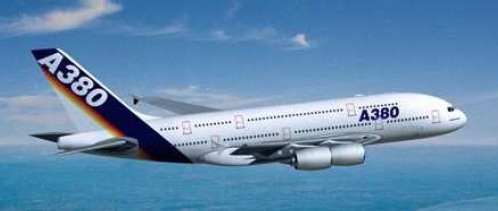
\includegraphics[width=.95\textwidth]{png/img1}
\end{center}
\end{minipage}\hfill
\begin{minipage}[c]{.6\linewidth}
\begin{center}
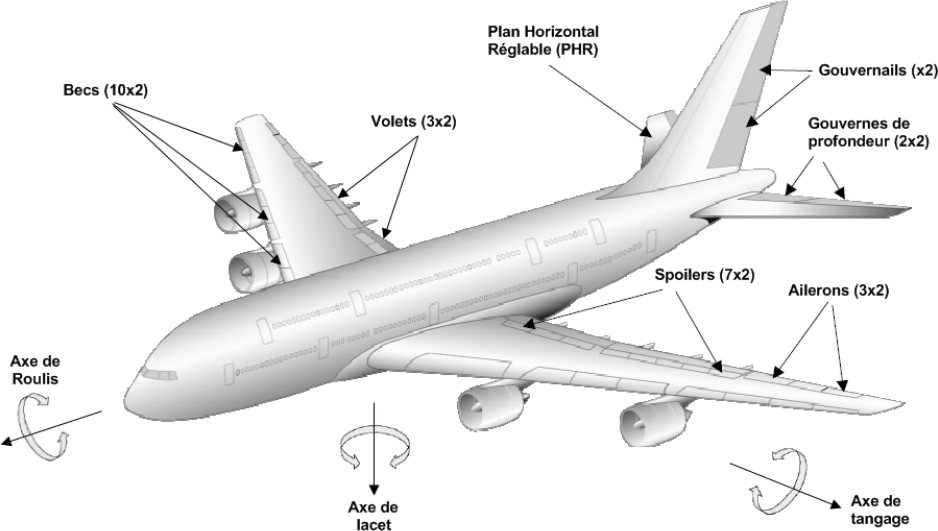
\includegraphics[width=.95\textwidth]{png/img2}
\end{center}
\end{minipage}

\vspace{.5cm}


Pour cela, le pilote agit sur les commandes de vol de l'avion. En pratique, on distingue deux types de commandes : 
\begin{itemize}
\item les commandes de vol primaires utilisées pendant tout le vol et qui permettent de contrôler l'évolution de l'avion autour de ses axes de référence :
\begin{itemize}
\item la gouverne de direction ou gouvernail pour le lacet;
\item les ailerons et les spoilers pour le roulis; 
\item les gouvernes de profondeur et le plan horizontal réglable (PHR) pour le tangage. 
\end{itemize}
\item Les commandes de vol secondaires utilisées pendant les phases d'atterrissage et de décollage qui permettent de modifier la configuration aérodynamique de l'avion :
\begin{itemize}
\item les hypersustentateurs (volets et becs) pour la portance;
\item les spoilers (ou aérofreins) pour la traînée.
\end{itemize}
\end{itemize}

L'airbus A380 est équipé de quatre gouvernes de profondeur disposées symétriquement sur le plan horizontal réglable (PHR) de l'avion. Chaque gouverne de profondeur est reliée au PHR par des charnières et est mis en rotation par une unité de commande constituée de deux actionneurs :
\begin{itemize}
\item une servocommande (SC), actionneur principal relié au circuit hydraulique de l'avion;
\item un EHA (Electro Hydraulic Actuator : actionneur électro-hydrostatique), utilisé comme organe de sécurité en cas de défaillance de la servocommande ou du circuit hydraulique principal.
\end{itemize}

Ces unités de commande sont identiques pour les quatre gouvernes de profondeur.


\begin{center}
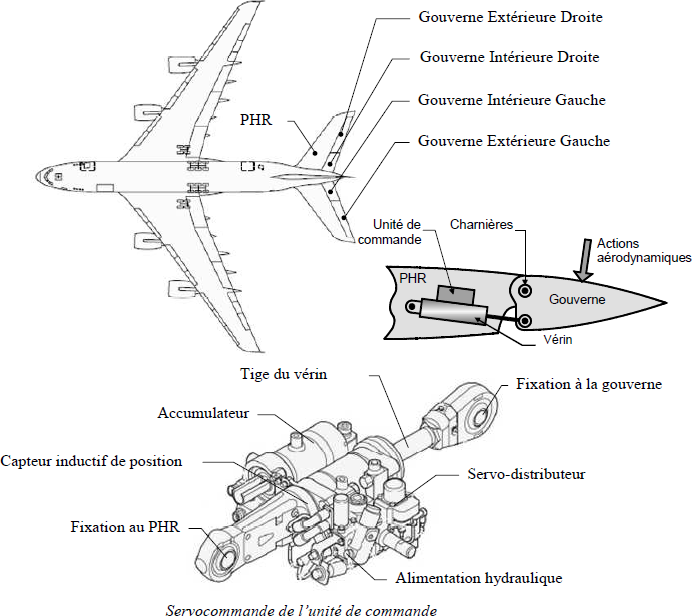
\includegraphics[width=.9\textwidth]{png/img3}
\end{center}
\begin{center}
\end{center}

Les consignes émises par le pilote à l'aide du joystick ou par le pilote automatique sont transmises aux ordinateurs de commande de vol. Ces derniers déterminent, en fonction de lois de pilotage prenant compte un certain nombre de paramètres (altitude, vitesse, etc.), les mouvements des gouvernes limitant éventuellement les évolutions de l'avion à son enveloppe de vol, c'est-à-dire aux régimes et altitudes sûrs.


\begin{center}
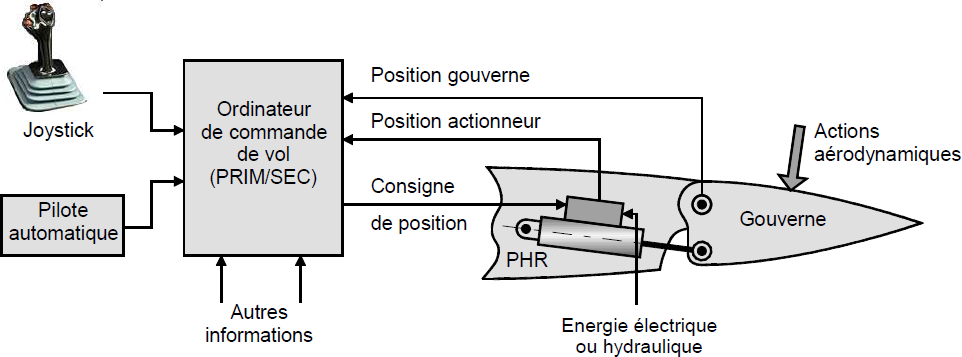
\includegraphics[width=.9\textwidth]{png/img4}
\end{center}

Le système peut être représenté par la chaîne topo fonctionnelle suivante : 
\begin{center}
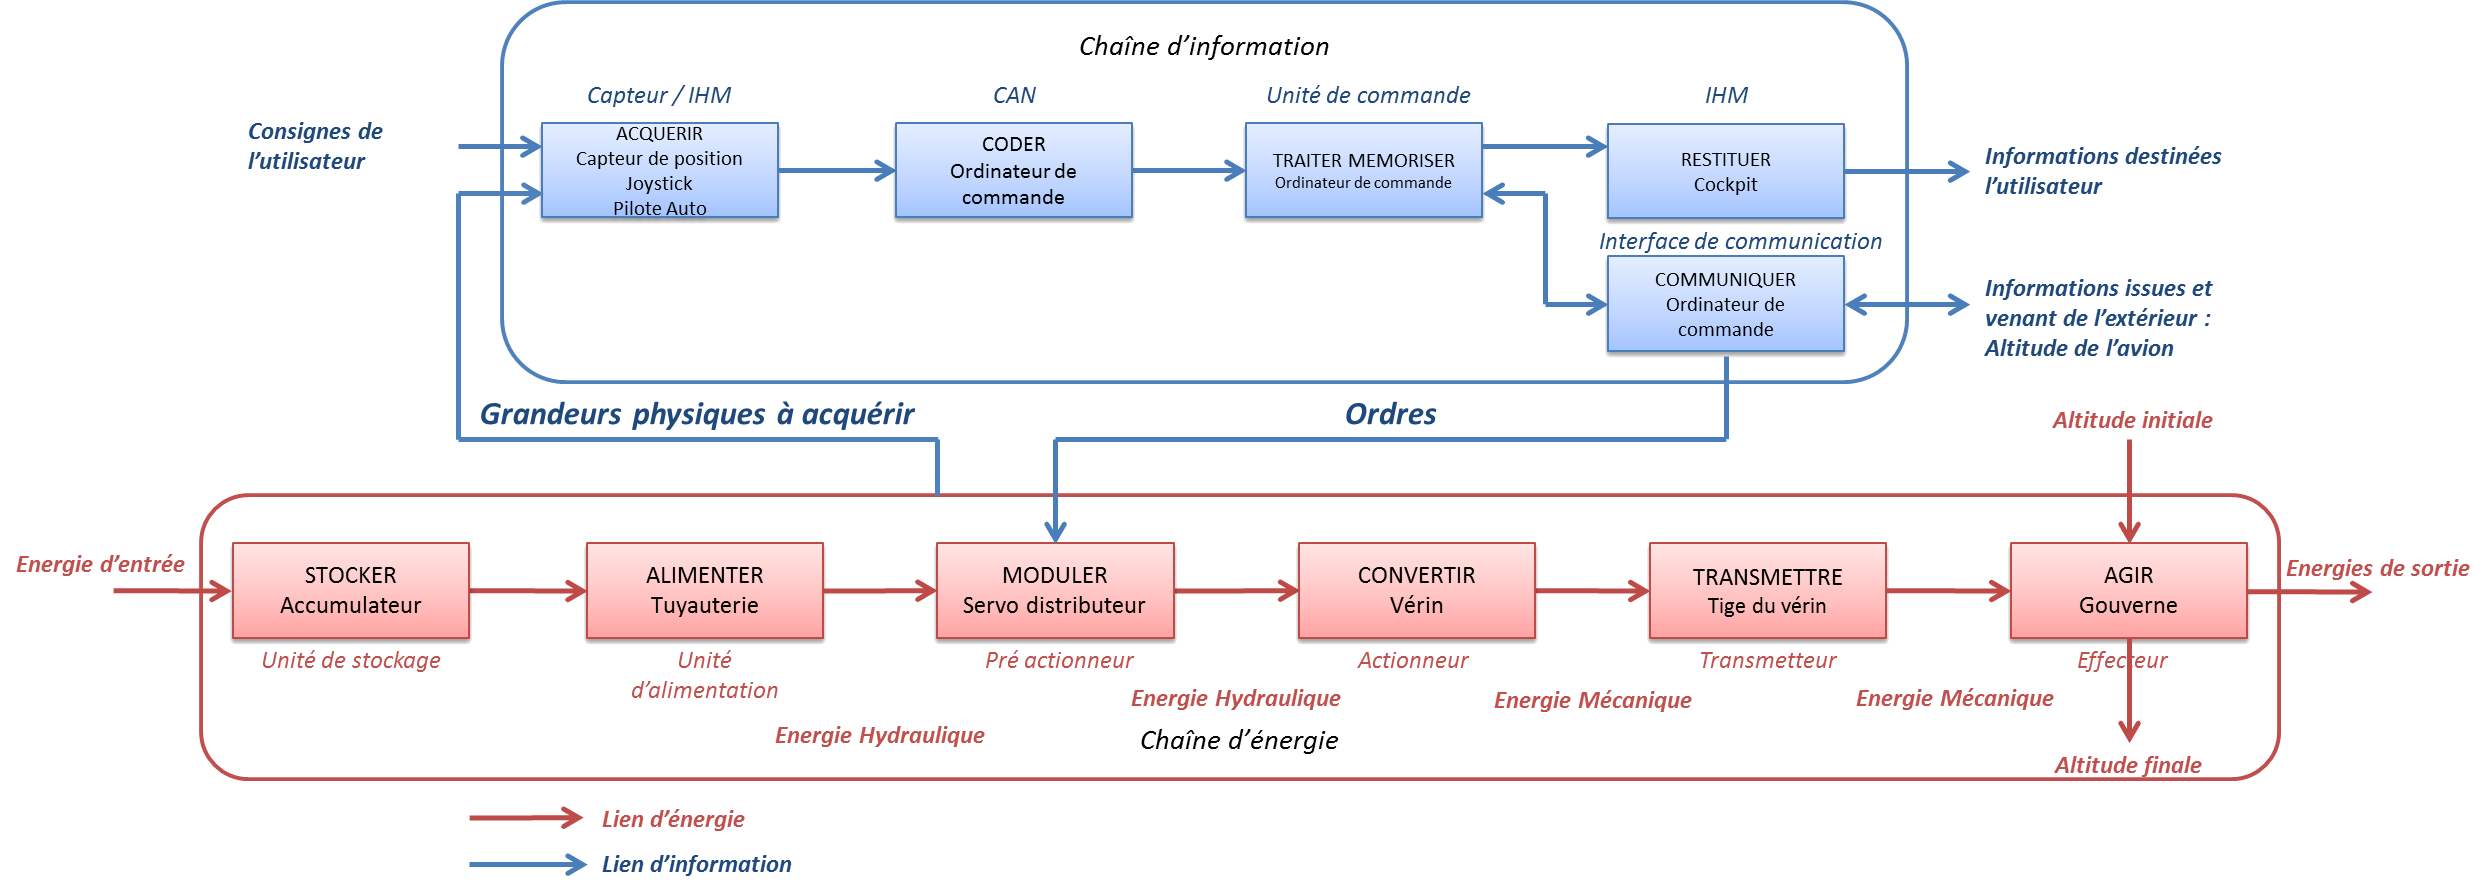
\includegraphics[width=\textwidth]{png/chaine}
\end{center}
}

\begin{minipage}{.5\linewidth}

On donne un diagramme des exigences partiel.
\begin{center}
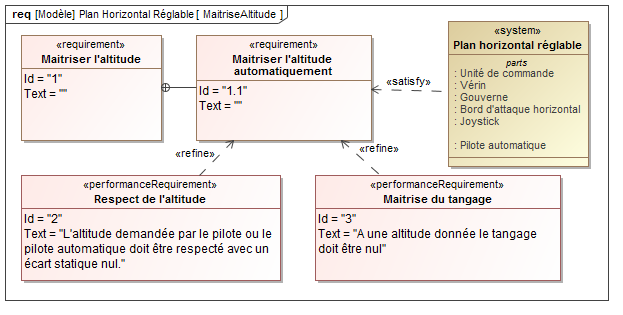
\includegraphics[width=\textwidth]{png/MaitriseAltitude}
\end{center}
\end{minipage}\hfill
\begin{minipage}{.47\linewidth}

\begin{obj}
L'objectif de ce TD est de vérifier que l'écart statique du système de maintien de l'altitude est nul.

\begin{center}
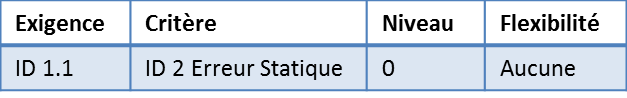
\includegraphics[width=\textwidth]{png/cdc}
\end{center}

\end{obj}
\end{minipage}

\subsection*{Étude de la servocommande}
\ifthenelse{\boolean{prof}}{}{

\begin{center}
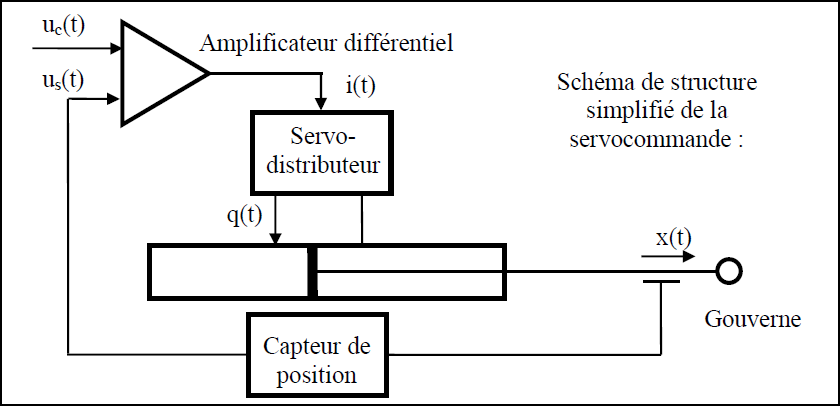
\includegraphics[width=.7\textwidth]{png/img5}
\end{center}

Les différentes équations temporelles qui modélisent le fonctionnement du système sont :
\begin{itemize}
\item un amplificateur différentiel défini par : $u_c(t)=\dfrac{i(t)}{K_a}+u_s(t)$;
\item débit dans le vérin dans le cas d'une hypothèse de fluide incompressible $q(t)=S\cdot\dfrac{dx(t)}{dt}$;
\item capteur de position : $u_s(t)=K_c\cdot x(t)$;
\item le servo-distributeur est un composant de la chaîne de commande conçu pour fournir un débit hydraulique $q(t)$ proportionnel au courant de commande $i(t)$. (Attention, valable uniquement en régime permanent.) Le constructeur fournit sa fonction de transfert :
$$
F(p)=\dfrac{Q(p)}{I(p)}=\dfrac{K_d}{1+Tp}
$$
où $K_d$ est le gain du servo-distributeur et $T$ sa constante de temps.
\end{itemize}
}





\subsection*{Modélisation dans l'hypothèse de fluide incompressible}
\subparagraph{}
\textit{Écrire les équations du modèle sous forme symbolique (transformée de Laplace) en considérant que toutes les conditions initiales sont nulles.}
\ifthenelse{\boolean{prof}}{
\begin{corrige}
On a :
\begin{itemize}
\item $U_c(p)=\dfrac{1}{K_a}I(p)+U_s(p)$
\item $Q(p)=SpX(p)$
\item $U_S(p)=K_C\cdot X(p)$
\item $F(p)=\dfrac{Q(p)}{I(p)}=\dfrac{K_d}{1+Tp}$
\end{itemize}
\end{corrige}
}{}

\subparagraph{}
\textit{Représenter chacune de ces relations sous forme de schéma bloc partiel.}
\ifthenelse{\boolean{prof}}{
\begin{corrige}

\begin{minipage}[c]{.23\linewidth}
\begin{center}
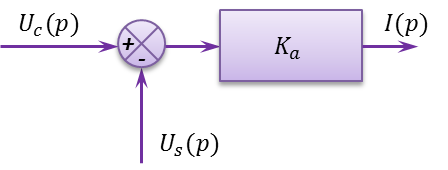
\includegraphics[width=.95\textwidth]{png/bloc1}
\end{center}
\end{minipage}\hfill
\begin{minipage}[c]{.23\linewidth}
\begin{center}
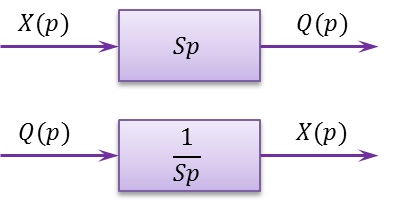
\includegraphics[width=.95\textwidth]{png/bloc2}
\end{center}
\end{minipage}\hfill
\begin{minipage}[c]{.23\linewidth}
\begin{center}
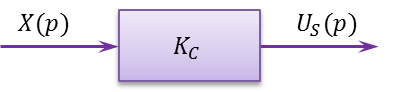
\includegraphics[width=.95\textwidth]{png/bloc3}
\end{center}
\end{minipage}\hfill
\begin{minipage}[c]{.23\linewidth}
\begin{center}
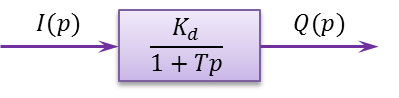
\includegraphics[width=.95\textwidth]{png/bloc4}
\end{center}
\end{minipage}


\end{corrige}
}{}

\subparagraph{}
\textit{Regrouper les schémas blocs partiels afin de représenter le schéma bloc correspondant au comportement de la servocommande.}
\ifthenelse{\boolean{prof}}{
\begin{corrige}
\begin{center}
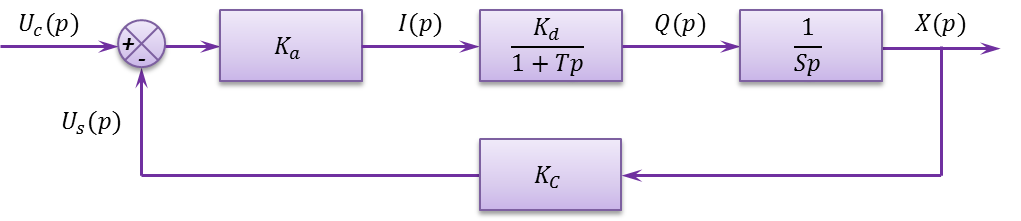
\includegraphics[width=.8\textwidth]{png/schema_bloc}
\end{center}
\end{corrige}
}{}

\subparagraph{}
\textit{Calculer les fonctions de transfert suivantes et donner à chaque fois la classe et l'ordre : 
\begin{itemize}
\item fonction de transfert du vérin non asservi : $A_1(p)=\dfrac{X(p)}{Q(p)}$;
\item fonction de transfert de la chaîne directe : $C(p)=\dfrac{X(p)}{\varepsilon(p)}$;
\item fonction de transfert boucle ouverte du système : $G(p)=\dfrac{U_s(p)}{\varepsilon(p)}$;
\item fonction de transfert en boucle fermée du système : $H(p)=\dfrac{X(p)}{U_c(p)}$.
\end{itemize}}
\ifthenelse{\boolean{prof}}{
\begin{corrige}
Fonction de transfert du vérin non asservi : 
$$A_1(p)=\dfrac{X(p)}{Q(p)} = \dfrac{1}{Sp}$$
$A_1(p)$ est d'ordre 1 et de classe 1.

Fonction de transfert de la chaîne directe : 
$$C(p)=\dfrac{X(p)}{\varepsilon(p)}= \dfrac{K_a\cdot K_d }{Sp\left( 1+Tp\right)}$$
$C(p)$ est d'ordre 2 et de classe 1.

Fonction de transfert boucle ouverte du système : 
$$G(p)=\dfrac{U_s(p)}{\varepsilon(p)}= \dfrac{K_a\cdot K_d \cdot K_C }{Sp\left( 1+Tp\right)}$$
$G(p)$ est d'ordre 2 et de classe 1.

Fonction de transfert en boucle fermée du système : 
$$H(p)=\dfrac{X(p)}{U_c(p)}
=\dfrac{\dfrac{K_a\cdot K_d }{Sp\left( 1+Tp\right)}}{1+\dfrac{K_a\cdot K_d \cdot K_C }{Sp\left( 1+Tp\right)}}
=\dfrac{K_a\cdot K_d }{Sp\left( 1+Tp\right)+K_a\cdot K_d \cdot K_C }
=\dfrac{\dfrac{K_a\cdot K_d}{K_a\cdot K_d \cdot K_C}}{\dfrac{Sp}{K_a\cdot K_d \cdot K_C}\left( 1+Tp\right)+1 }
$$
$H(p)$ est d'ordre 2 et de classe 0.
\end{corrige}
}{}

\subparagraph{}
\textit{Le système étant régit par sa fonction transfert en boucle fermée, déterminer, dans le domaine temporel, la réponse indicielle du système.}
\ifthenelse{\boolean{prof}}{
\begin{corrige}

\end{corrige}
}{}


\subparagraph{}
\textit{Dans le cas d'un échelon, donner la valeur initiale, la valeur finale et la pente à l'origine de la sortie.}
\ifthenelse{\boolean{prof}}{
\begin{corrige}
\end{corrige}
}{}

\subparagraph{}
\textit{Déterminer l'écart statique.}
\ifthenelse{\boolean{prof}}{
\begin{corrige}
Dans la configuration, donnée, l'entrée et la sortie du système ne sont pas les mêmes grandeurs physiques. En conséquence, l'écart statique peut être défini par : 
$$
\varepsilon_S 
= \lim\limits_{t\to+\infty} \varepsilon(t)
= \lim\limits_{p\to 0} p\varepsilon(p)
= \lim\limits_{p\to 0} p\dfrac{E(p)}{1+C(p)}
$$

$E(p)$ étant une entrée indicielle, l'entrée est un échelon d'amplitude 1; donc $E(p)=\dfrac{1}{p}$.
$$
\varepsilon_S 
= \lim\limits_{p\to 0} p\dfrac{1}{p}\dfrac{1}{1+\dfrac{K_a\cdot K_d }{Sp\left( 1+Tp\right)}}
= \lim\limits_{p\to 0} \dfrac{Sp\left( 1+Tp\right)}{Sp\left( 1+Tp\right)+K_a\cdot K_d}
= 0
$$
\end{corrige}
}{}

\subparagraph{}
\textit{Conclure quant à la validité du cahier des charges dans le cas où le fluide est incompressible.}
\ifthenelse{\boolean{prof}}{
\begin{corrige}
Dans le cas où on fait l'hypothèse que le fluide n'est pas compressible, l'écart statique est nul. Le cahier des charges est donc vérifié.
\end{corrige}
}{}


\subsection*{Modélisation dans l'hypothèse du fluide compressible}
Dans cette hypothèse, le modèle de connaissance du système est modifié : 
\begin{itemize}
\item l'équation de débit dans le vérin devient : $q(t)=S\cdot\dfrac{dx(t)}{dt}+\dfrac{V}{2B}\dfrac{d\Delta p(t)}{dt}$ où $\Delta p(t)$ représente la différence de pression entre les 2 chambres du vérin, $V$ est le volume total de fluide dans le vérin ($V$ est constant) et $B$ le coefficient de compressibilité du fluide hydraulique (pour un fluide incompressible $B\rightarrow \infty$);
\item effort moteur sur le piston : $F_m(t)=S\cdot \Delta p(t)$;
\item principal fondamental de la dynamique appliqué sur la tige de vérin :
$F_m(t)-F_r(t)-f\dfrac{dx(t)}{dt}=m\cdot\dfrac{d^2x(t)}{dt^2}$ où $F_r(t)$ représente l'effort résistant sur la tige du vérin, effort qui sera considéré comme une perturbation et $f$ représente le frottement visqueux.
\end{itemize}

\subparagraph{}
\textit{Écrire les équation du modèle sous forme symbolique (transformée de Laplace) en considérant que toutes les conditions initiales sont nulles.}
\ifthenelse{\boolean{prof}}{
\begin{corrige}
On a :
\begin{itemize}
\item $Q(p)=S\cdot pX(p)+\dfrac{V}{2B}p \Delta P(p)$;
\item $F_m(p)=S\cdot \Delta P(p)$;
\item $F_m(p)-F_r(p)-fpX(p)=m\cdot p^2 X(p)$.
\end{itemize}

\end{corrige}
}{}

\subparagraph{}
\textit{Représenter chacune de ces relations sous forme de schéma bloc partiel.}
\ifthenelse{\boolean{prof}}{
\begin{corrige}
\begin{minipage}[c]{.3\linewidth}
\begin{center}
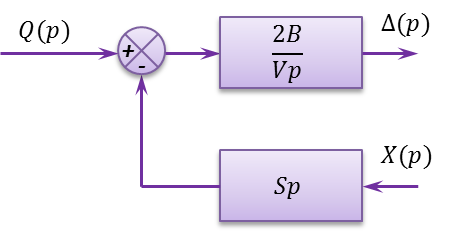
\includegraphics[width=.95\textwidth]{png/bloc5}
\end{center}
\end{minipage}\hfill
\begin{minipage}[c]{.3\linewidth}
\begin{center}
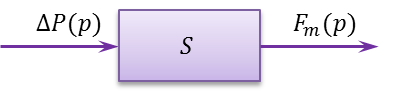
\includegraphics[width=.95\textwidth]{png/bloc6}
\end{center}
\end{minipage}\hfill
\begin{minipage}[c]{.3\linewidth}
\begin{center}
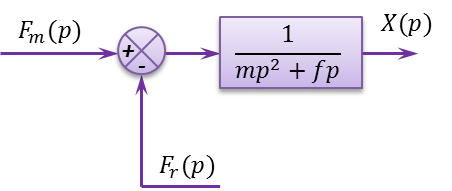
\includegraphics[width=.95\textwidth]{png/bloc7}
\end{center}
\end{minipage}

\end{corrige}
}{}

\subparagraph{}
\textit{Regrouper les schémas-blocs partiels. Afin de représenter le comportement du vérin non asservi (grandeur d'entrée $Q(p)$, grandeur de sortie $X(p)$). Le schéma bloc contiendra un retour et une perturbation.}
\ifthenelse{\boolean{prof}}{
\begin{corrige}
\begin{center}
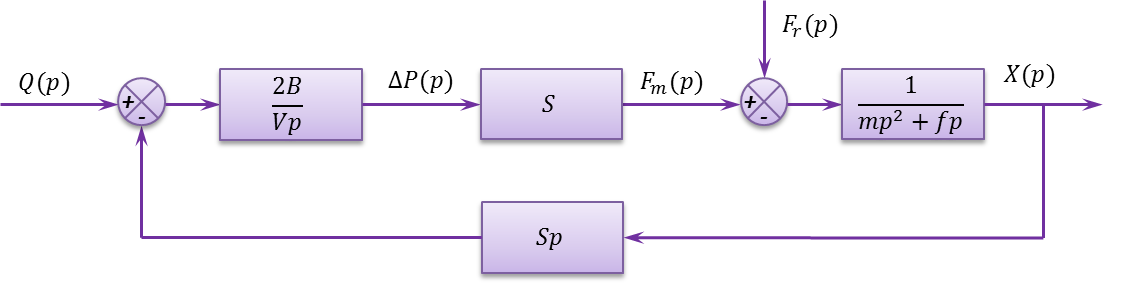
\includegraphics[width=.8\textwidth]{png/schema_bloc_2}
\end{center}
\end{corrige}
}{}

\subparagraph{}
\textit{Calculer la nouvelle fonction de transfert du vérin non asservi : $A_2(p)=\dfrac{X(p)}{Q(p)}$, en supposant que la perturbation $F_r(t)$ est nulle. Donner à chaque fois la classe et l'ordre de $A_2(p)$.}
\ifthenelse{\boolean{prof}}{
\begin{corrige}
On a : 
$$A_2(p)
=\dfrac{X(p)}{Q(p)}
=\dfrac{\dfrac{2B}{Vp}\cdot S\cdot\dfrac{1}{mp^2+fp}}{1+\dfrac{2B}{Vp}\cdot S\cdot\dfrac{1}{mp^2+fp}\cdot Sp}
=\dfrac{2BS}{mVp^3+fVp^2+2BS^2p}
$$

$$A_2(p)
=\dfrac{1}{p}\cdot\dfrac{2BS}{mVp^2+fVp+2BS^2}
$$

Cette fonction de transfert est d'ordre 3 et de classe 1.
\end{corrige}
}{}

\subparagraph{}
\textit{Donner la fonction de transfert du système complet dans le cas où $Q(p)$ est non nulle et $F_r(p)$  est nulle.}
\ifthenelse{\boolean{prof}}{
\begin{corrige}
\end{corrige}
}{}

\subparagraph{}
\textit{Quelle est la modification apportée par le modèle du fluide incompressible.}
\ifthenelse{\boolean{prof}}{
\begin{corrige}
\end{corrige}
}{}

\subparagraph{}
\textit{Calculer l'écart statique et conclure quant à la validité du cahier des charges dans le cas où le fluide est considéré comme compressible et que $F_r(p)$ est nulle.}
\ifthenelse{\boolean{prof}}{
\begin{corrige}
\end{corrige}
}{}

\subparagraph{}
\textit{Exprimer $X(p)$ en fonction de $U_C(p)$ et $F_r(p)$.}
\ifthenelse{\boolean{prof}}{
\begin{corrige}
\end{corrige}
}{}

\subparagraph{}
\textit{Le cahier des charges est-il vérifié lorsque les deux entrées sont des échelons d'amplitude 1 ?}
\ifthenelse{\boolean{prof}}{
\begin{corrige}
\end{corrige}
}{}


\end{document}


\subparagraph{}
\textit{Conclure sur la validité du cahier des charges.}

\ifthenelse{\boolean{prof}}{
\begin{corrige}
On observe que le système a un écart statique nul : la consigne était de $1\; rad$ et l'angle atteint par l'axe de lacet est de $1\; rad$. Le critère d'écart statique est donc vérifié. 

En revanche, on observe un léger dépassement de la consigne. En conséquence, le critère de dépassement nul n'est pas vérifié. 
\end{corrige}
}{}
\end{document}
